\section{Hypothesis-Driven Research Extension}
\subsection{From Replication to a Discriminating Question}
The localization experiments above reproduce established TFEB biology. The extension asks a different question: \textit{does the transcriptional effect of the C-terminal S466/S467/S469 cluster depend on the stimulus and on fusion to EGFP, after accounting for protein abundance and nuclear exposure?} A tag effect is a hypothesis to test, not an explanation already established by the literature.

Paquette et al. reported that the S466A/S467A/S469A mutant (3A) could accumulate in nuclei yet showed impaired transcriptional activity in their experimental systems; they also examined combinations with S142A/S211A \cite{Paquette2021}. Negoita et al. subsequently observed AMPK-associated dephosphorylation of this cluster and explicitly raised the possibility that alanine substitutions affect local structure as well as phosphorylation \cite{Negoita2026}. Their study also distinguished AMPK-dependent responses to MK-8722 from responses to Torin1. Different cell systems, stimuli and constructs prevent treating these findings as a single matched comparison. Neither 3A nor the five-site alanine combination is a new mutant invented here.

Our proposed contribution is a controlled genotype--tag--stimulus comparison in HeLa cells, followed by selected mechanistic tests. The 3T substitution retains hydroxyl-bearing side chains but remains potentially phosphorylatable; it is a sequence/chemistry probe, not a constitutively dephosphorylated mimic. A targeted literature search supports this rationale but does not establish that the exact combination has never been tested. No claim of first discovery is made.

\subsection{Five Additional Sequence-Defined Constructs}
The existing WT fusion is reused. Five additional plasmid designs provide the remaining cells of the six-construct matrix (Table~\ref{tab:research-constructs}). All retain the same CMV promoter and bacterial backbone. Full GenBank, DNA FASTA and translated protein files are supplied in \texttt{research-v3}; circular maps are shown in Figures~\ref{fig:research-tagged} and~\ref{fig:research-untagged}.

\begin{table}[htbp]\centering\small
\caption{Research constructs and exact intended changes. Coordinates refer to the accepted 6,134-bp WT fusion.}\label{tab:research-constructs}
\begin{tabularx}{\textwidth}{L{0.27\textwidth}L{0.13\textwidth}Y}
\toprule Construct & bp / aa & Intended difference from the WT fusion \\
\midrule
3A--EGFP & 6134 / 722 & S466A/S467A/S469A; each AGC codon becomes GCC. \\
3T--EGFP & 6134 / 722 & S466T/S467T/S469T; each AGC codon becomes ACC. \\
WT, untagged & 5396 / 476 & Replace bp 2059--2799 (linker plus EGFP including stop) with the native TFEB stop codon TGA. \\
3A, untagged & 5396 / 476 & The same tag removal plus the three AGC-to-GCC changes. \\
3T, untagged & 5396 / 476 & The same tag removal plus the three AGC-to-ACC changes. \\
\bottomrule
\end{tabularx}
\end{table}

The three codons occupy bp 2026--2028, 2029--2031 and 2035--2037; intervening F468 is unchanged. Tag removal shortens the plasmid by 738 bp and eliminates the original BamHI site. Therefore the WT HindIII/BamHI diagnostic and its expected fragment sizes cannot be reused for untagged constructs. For this extension, the proposed procurement route is sequence-defined whole-plasmid synthesis followed by independent whole-plasmid sequence verification, including every altered codon, the new stop junction and the backbone. No order has been placed and no assembly primers have been experimentally validated. Two independently recovered, sequence-accepted bacterial clones per construct will confirm key comparisons; they are not counted as independent culture-day replicates.

\begin{figure}[htbp]\centering
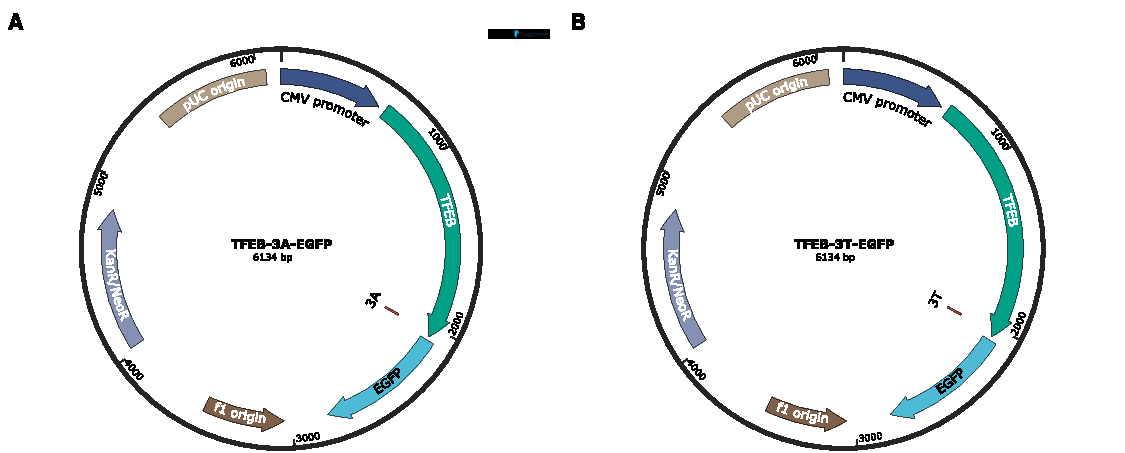
\includegraphics[width=\textwidth]{images/B/research-tagged-plasmids.pdf}
\caption{Additional tagged constructs rendered by SnapGene Viewer. (A) TFEB-3A--EGFP; (B) TFEB-3T--EGFP. Both are 6,134 bp. The red feature marks the S466/S467/S469 cluster; its span includes unchanged intervening sequence. CMV is blue, TFEB teal, EGFP cyan, selection purple and replication origins brown. Maps show sequence designs, not experimentally recovered plasmids.}
\label{fig:research-tagged}
\end{figure}

\begin{figure}[htbp]\centering
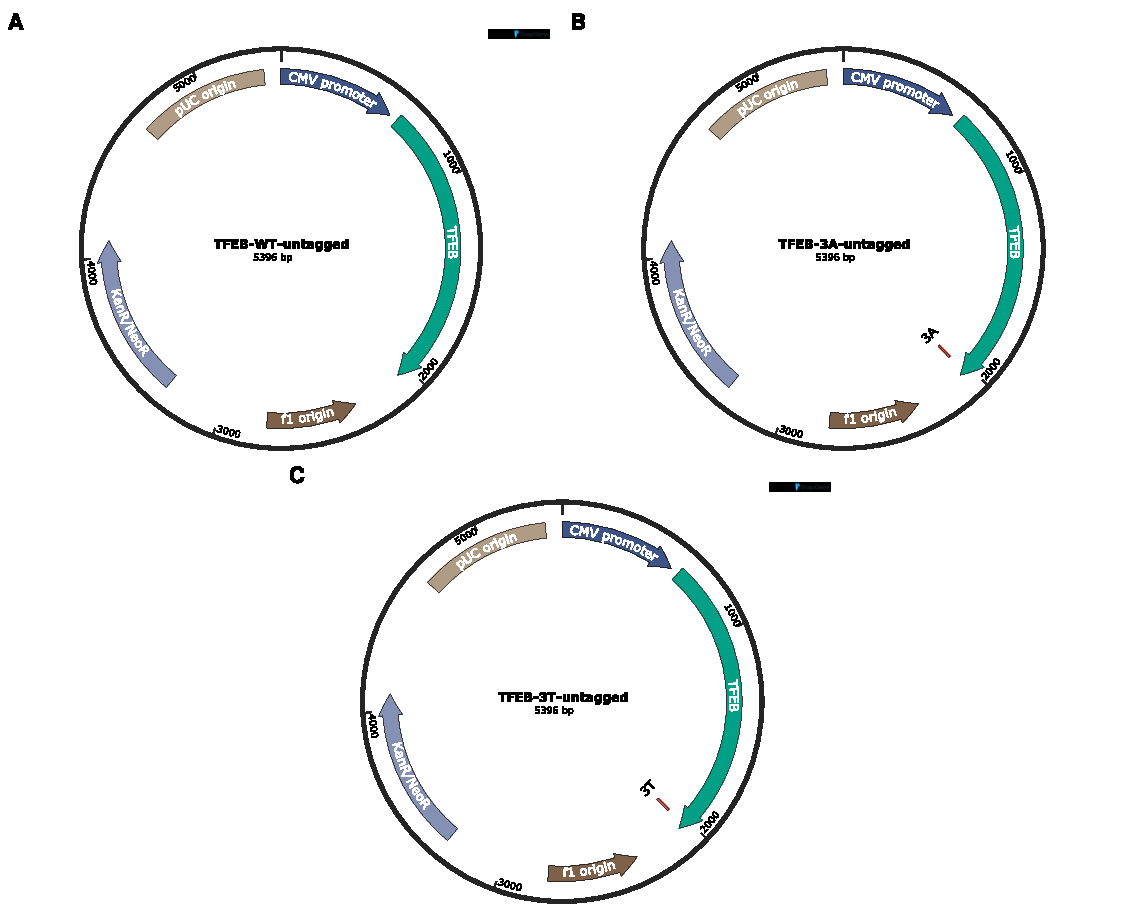
\includegraphics[width=\textwidth]{images/B/research-untagged-plasmids.pdf}
\caption{Matched untagged constructs rendered by SnapGene Viewer: (A) WT, (B) 3A and (C) 3T. Each is 5,396 bp and encodes a 476-residue TFEB protein followed by its native stop codon. Removing the linker and EGFP preserves the remainder of the parental backbone while changing downstream coordinates and the restriction pattern. Feature colors match the tagged maps. Full annotations and independent sequence checks accompany the design files.}
\label{fig:research-untagged}
\end{figure}
\FloatBarrier

\subsection{Core Factorial Comparison and Controls}
Cross WT/3A/3T with EGFP-tagged/untagged TFEB and vehicle/Torin1/MK-8722, yielding 18 core conditions (Figure~\ref{fig:research-design}). Perform the principal rescue comparison after endogenous TFEB depletion with a validated 3$'$-UTR siRNA that does not target these coding-only constructs. Repeat the decisive contrasts with a second individual TFEB siRNA. Non-targeting siRNA, mock transfection, depleted cells without rescue and matched EGFP-only controls are additional arms, not part of the 18-condition count. Confirm depletion of endogenous transcript using a 3$'$-UTR assay and quantify residual endogenous protein; the untagged rescue cannot be distinguished from endogenous TFEB by size alone.

Pilot DNA amounts separately to overlap total TFEB abundance and the fraction of expressing cells across constructs, using matched total DNA and transfection reagent. Do not assume equal DNA produces equal protein. Quantify tagged and untagged proteins with the same validated anti-TFEB reagent recognizing an epitope outside the altered C-terminal region. Validate its response using TFEB depletion and equivalent antigen loading. Analyze randomly selected fields with a preregistered expression threshold anchored to depleted/no-rescue controls; report all-cell and expression-stratified results and the fraction excluded. Do not select only bright GFP-positive cells in one arm. Bulk RT-qPCR comparisons require comparable expressing-cell fractions as well as comparable abundance; otherwise report this confounding and revise the transfection system before interpreting a tag effect.

For the extension, use a common nutrient-replete medium and matched final solvent in every treatment. Pilot MK-8722 at 1, 3 and 10~$\mu$M and retain the lowest tolerated dose with clear ACC phosphorylation; retain the established Torin1 pilot range. These are proposed HeLa starting points, not validated operating conditions. Verify AMPK engagement with p-ACC/total ACC and mTORC1 inhibition with p-S6K/total S6K, together with TFEB abundance, cell number and viability. Monitor localization at 0, 30, 60 and 120 min using matched plates and collect RNA at 6 h; include a 6-h localization/abundance check so an early nuclear snapshot is not treated as equivalent nuclear exposure throughout transcription. The final schedule and dose are fixed after the pilot and before confirmatory analysis.

\begin{figure}[htbp]\centering
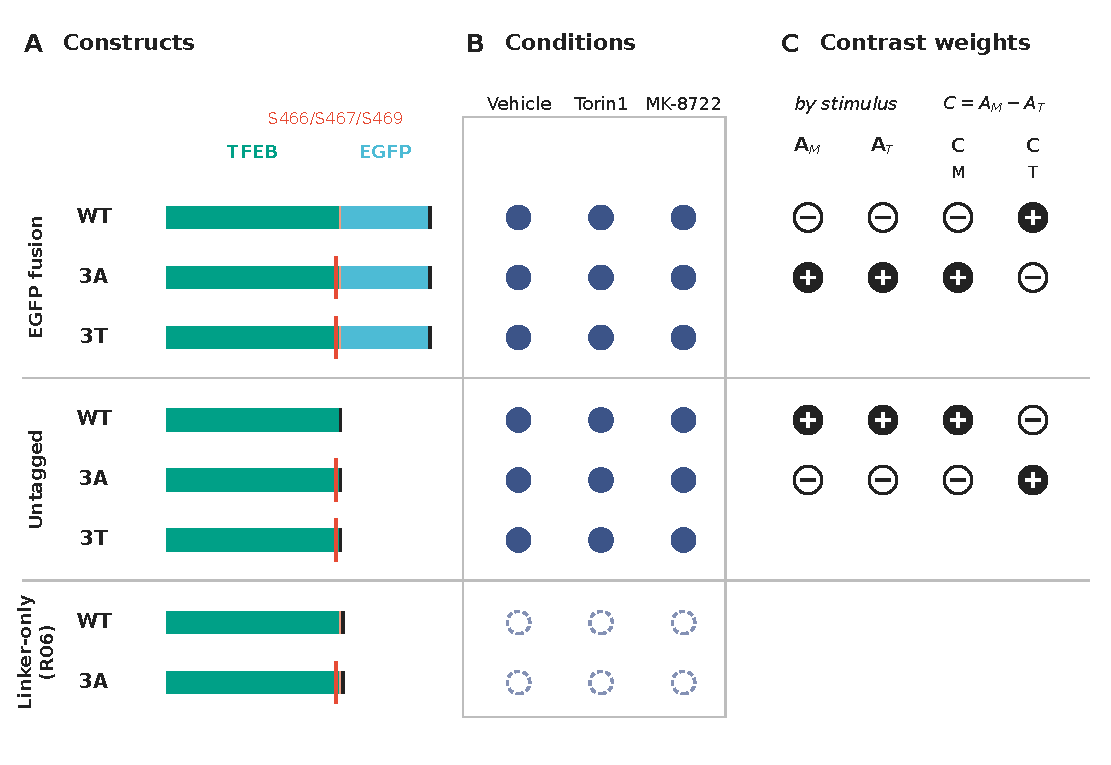
\includegraphics[width=\textwidth]{images/B/research-design.pdf}
\caption{Factorial design for the research extension. (A) WT, 3A and 3T TFEB are compared with the existing C-terminal EGFP fusion architecture (upper three rows) or without the linker/tag (lower three rows). Red ticks mark the altered C-terminal cluster; the schematic omits small sequence features. (B) Each row is crossed with vehicle, Torin1 and MK-8722, giving 18 core conditions. Open circles represent planned experimental conditions, not data points or replicates. Localization, transcription and phosphorylation are separate readouts. TFEB-depletion/rescue controls, solvent matching, expression checks and additional genetic controls are specified in the text.}
\label{fig:research-design}
\end{figure}

Use normalized MCOLN1 transcript abundance at 6 h as the primary functional endpoint; LAMP1 and CTSD are secondary endpoints after primer-efficiency and reference-gene validation. Average technical wells within each independent culture day. For each tag and drug, calculate the 3A-versus-WT difference in drug-induced log$_2$ expression relative to its own vehicle. The prespecified primary contrast compares the tagged-minus-untagged difference between MK-8722 and Torin1, i.e. a genotype--tag--stimulus interaction. Report its effect estimate and confidence interval with the underlying component contrasts; apply Holm adjustment to the prespecified secondary contrast family. 3T comparisons are exploratory. Start planning with four independent days, then determine confirmatory sample size from an independent pilot and a biologically meaningful target precision; four days alone do not establish adequate power. Analyze localization and abundance alongside transcription, rather than declaring a direct transcriptional defect from a lower qPCR signal alone.

\subsection{Mechanistic Follow-Up with Defined Decision Rules}
\textbf{AMPK dependence.} In the most informative WT/3A comparison, co-deplete PRKAA1 and PRKAA2 using two independent siRNA pairs in separate experiments. Include non-targeting siRNA, single-target checks, mock controls and both drugs. Verify both catalytic-subunit reductions and loss of MK-8722-induced p-ACC, plus viability and rescue abundance. A selective loss of the MK-8722 response with a retained Torin1 response would support stimulus-dependent AMPK involvement. It would not identify the enzyme acting directly on the TFEB cluster. Failed target engagement makes a negative result uninterpretable. Exact siRNA sequences and off-target checks remain prerequisites.

\textbf{Phosphosite specificity.} In WT tagged and untagged samples, measure C-terminal phosphorylation together with total TFEB at baseline and after treatment. Phospho-antibodies require phosphatase-treated material, unmodified/phosphorylated peptide controls and site-mutant controls; adjacent residues can affect epitope recognition. Loss of signal in 3A alone is not evidence of physiological dephosphorylation. If specificity is unresolved, use targeted LC--MS/MS with site-localization evidence and total-protein normalization, reporting ambiguous adjacent-site assignments as such. Analyze any threonine phosphorylation in 3T by an appropriate assay; a serine-phospho-antibody cannot establish its state. This analytical follow-up is conditional on instrument access and assay development.

\textbf{Promoter engagement.} If transcription differs despite comparable nuclear exposure and abundance, test TFEB occupancy near validated MCOLN1 and LAMP1 regulatory regions by ChIP--qPCR. Include input, matched IgG, TFEB-depleted/no-rescue material and a negative genomic region; validate antibody specificity and amplicons before use. Reduced occupancy would suggest altered promoter engagement. Comparable occupancy with different transcription would motivate later cofactor studies, without proving a particular cofactor mechanism. If localization or abundance differs, resolve that upstream explanation before assigning a direct transactivation effect.

\begin{table}[htbp]\centering\small
\caption{Interpretive boundaries of possible extension outcomes; all outcomes are hypothetical.}\label{tab:research-decisions}
\begin{tabularx}{\textwidth}{L{0.36\textwidth}Y}
\toprule Observed pattern, if obtained & Supported interpretation and remaining alternative \\
\midrule
3A defect only in EGFP-tagged TFEB & Supports a tag-dependent effect under the tested conditions; expression, antibody and delivery differences must be excluded. \\
3A defect in both tag states & A tag alone is insufficient to explain the effect; phosphorylation and local structural changes remain alternatives. \\
3T resembles WT while 3A differs & Consistent with a contribution of local side-chain chemistry; 3T phosphorylation must be measured before attributing the difference to hydroxyl retention alone. \\
Different effects under Torin1 and MK-8722 & Supports stimulus dependence after verified pathway engagement; does not identify a direct kinase or phosphatase. \\
Nuclear exposure or abundance also differs & Transcriptional differences cannot yet be assigned to intrinsic transactivation. \\
No clear interaction with wide intervals & Inconclusive precision, not evidence that tags or sites have no effect. \\
\bottomrule
\end{tabularx}
\end{table}

\subsection{Additional Workload and Feasibility}
The extension adds five modules after the core M01--M12 program: R01, verify the five new constructs and expression matching; R02, execute the 18-condition comparison; R03, test AMPK dependence; R04, resolve phosphosite specificity; and R05, test promoter occupancy if its entry criterion is met. R01--R03 may be scheduled provisionally in weeks 9--12 after reagent availability. R04--R05 are conditional follow-ups whose completion depends on assay development and access; the eight-week core plan does not include their full execution.

At four independent days and two technical wells, the 18-condition matrix requires 144 wells \emph{per assay and endpoint}, before controls, pilot plates, additional time points or second-siRNA validation. Separate destructive IF, protein and RNA collections need separate samples. Each module must deliver raw records, exclusions and effect estimates, including failed or null comparisons. This increases assessable experimental work while keeping replication, hypothesis testing and unresolved implementation requirements distinguishable.
\FloatBarrier
